\documentclass[a4paper, 12pt, reqno]{article}
\linespread{1.1}
\usepackage{listings}             % Include the listings-package
\usepackage{xcolor}
\usepackage{graphicx}
\usepackage{float}
\usepackage{amsmath,mathtools,amsthm,amsfonts,amssymb,latexsym,bm}
\usepackage{mathrsfs}
\usepackage{natbib}
\usepackage{textcomp}
\usepackage{gensymb, multicol}
\usepackage{hyperref}

\definecolor{codegreen}{rgb}{0,0.6,0}
\definecolor{codegray}{rgb}{0.5,0.5,0.5}
\definecolor{codepurple}{rgb}{0.58,0,0.82}
\definecolor{backcolour}{rgb}{255,255,255}

\lstdefinestyle{mystyle}{
    backgroundcolor=\color{backcolour},   
    commentstyle=\color{codegreen},
    keywordstyle=\color{magenta},
    numberstyle=\tiny\color{codegray},
    stringstyle=\color{codepurple},
    basicstyle=\ttfamily\footnotesize,
    breakatwhitespace=false,         
    breaklines=true,                 
    captionpos=b,                    
    keepspaces=true,                 
    numbers=left,                    
    numbersep=5pt,                  
    showspaces=false,                
    showstringspaces=false,
    showtabs=false,                  
    tabsize=2
}

\lstset{style=mystyle}
\lstset{language=Python}

\renewcommand{\thesection}{}%
\renewcommand{\thesubsection}{}%
\newcommand{\ro}[1]{%
  \xrightarrow{\mathmakebox[\rowidth]{#1}}%
}
\newlength{\rowidth}% row operation width
\AtBeginDocument{\setlength{\rowidth}{3em}}


\usepackage{blindtext}
\title{EBA3650: Quantitative economics}
\date{\today}
\author{Pauline Malaguti}





\begin{document}

\maketitle

This file was created to contain explanations and code examples for the course EBA3650 Quantitative Economics at BI Norwegian Business School.

\tableofcontents

\newpage
\section{Root Finding}
Root finding refers to the general problem of searching for a solution of an equation $F(x) = 0$  for some function $F$.  
If we want to optimise a function $f(x)$ then we need to find critical points and therefore solve the equation  $f'(x)= 0$. \\
Example quadratic formula: \\
\begin{equation}
x = \frac{-b \pm \sqrt{b^2 - 4ac}}{2a}
\notag
\end{equation}

\href{https://personal.math.ubc.ca/~pwalls/math-python/roots-optimization/root-finding/}{Source}

\section{Bisection Method}
The algorithm applies to any continuous function $f(x)$ on an interval a,b where the value of the function $f(x)$ changes sign from $a$ to $b$ . The idea is simple: divide the interval in two, a solution must exist within one subinterval, select the subinterval where the sign of $f(x)$ changes and repeat. \\
\subsection{Algorithm}
The bisection method procedure is:
\begin{enumerate}
  \item Choose a starting interval $[a_0,b_0]$ such that $f(a_0)f(b_0)<0$
  \item Compute $f(m_0)$ where $m_0=(a_0+b_0)/2$ is the midpoint.
  \item Determine the next subinterval $[a_1,b_1]$ :
	\begin{enumerate}
       \item If $f(a_0)f(m_0)<0$, then let $[a_1,b_1]$  be the next interval with $a_1=a_0$ and $b_1=m_0$.
       \item If $f(b_0)f(m_0)<0$, then let $[a_1,b_1]$  be the next interval with $a_1=m_0$ and $b_1=b_0$.
	\end{enumerate}
\item Repeat (2) and (3) until the interval $[a_N,b_N]$ reaches some predetermined length.
\item Return the midpoint value $m_N=(a_N+b_N)/2$
\end{enumerate}
A solution of the equation $f(x)$ on an interval a,b is guaranteed by the \underline{Intermediate Value Theorem} provided $f(x)$ is continuous on $[a,b]$ and \\$f(a)f(b)<0$. In other words, the function changes sign over the interval and therefore must equal 0 at some point in the interval $[a,b]$.
\subsection{Python Implementation}
Write a function called \texttt{bisection} which takes 4 input parameters \texttt{f, a, b} and \texttt{N} and returns the approximation of a solution of $f(x)=0$ given by N iterations of the bisection method. If  $f(a_N)f(b_N)>0$ at any point in the iteration (caused either by a bad initial interval or rounding error in computations), then print "\texttt{Bisection method fails.}" and return \texttt{None}.
\begin{lstlisting}[frame=single]  % Start your code-block
x
def bisection(f,a,b,N):
    '''Approximate solution of f(x)=0 on interval [a,b] by bisection method.

    Parameters
    ----------
    f : function
        The function for which we are trying to approximate a solution f(x)=0.
    a,b : numbers
        The interval in which to search for a solution. The function returns
        None if f(a)*f(b) >= 0 since a solution is not guaranteed.
    N : (positive) integer
        The number of iterations to implement.

    Returns
    -------
    x_N : number
        The midpoint of the Nth interval computed by the bisection method. The
        initial interval [a_0,b_0] is given by [a,b]. If f(m_n) == 0 for some
        midpoint m_n = (a_n + b_n)/2, then the function returns this solution.
        If all signs of values f(a_n), f(b_n) and f(m_n) are the same at any
        iteration, the bisection method fails and return None.

    Examples
    --------
    >>> f = lambda x: x**2 - x - 1
    >>> bisection(f,1,2,25)
    1.618033990263939
    >>> f = lambda x: (2*x - 1)*(x - 3)
    >>> bisection(f,0,1,10)
    0.5
    '''
    if f(a)*f(b) >= 0:
        print("Bisection method fails.")
        return None
    a_n = a
    b_n = b
    for n in range(1,N+1):
        m_n = (a_n + b_n)/2
        f_m_n = f(m_n)
        if f(a_n)*f_m_n < 0:
            a_n = a_n
            b_n = m_n
        elif f(b_n)*f_m_n < 0:
            a_n = m_n
            b_n = b_n
        elif f_m_n == 0:
            print("Found exact solution.")
            return m_n
        else:
            print("Bisection method fails.")
            return None
    return (a_n + b_n)/2


\end{lstlisting}

\href{https://personal.math.ubc.ca/~pwalls/math-python/roots-optimization/bisection/}{Source}


\section{Secant method}
The secant method is very similar to the bisection method except instead of dividing each interval by choosing the midpoint the secant method divides each interval by the secant line connecting the endpoints. The secant method always converges to a root of $f(x)$ is continuous on $[a,b]$ and $f(a)f(b)<0$.

\subsection{Secant line formula}
Let $f(x)$ be a continuous function on $[a,b]$ and $f(a)f(b)<0$. A solution of the equation $f(x) = 0$ for $x \in [a,b]$ is guaranteed by the \underline{Intermediate Value} \underline{Theorem}. Consider the line connecting the endpoint values $(a,f(a))$ and $(b,f(b))$. The line connecting these two points is called the secant line and is given by the formula
\begin{equation}
y = \frac{f(b) - f(a)}{b - a}(x - a) + f(a)
\notag
\end{equation}
The point where the secant line crosses the $x$-axis is
\begin{equation}
0 = \frac{f(b) - f(a)}{b - a}(x - a) + f(a)
\notag
\end{equation}
which we solve for $x$
\begin{equation}
x = a - f(a)\frac{b - a}{f(b) - f(a)}
\notag
\end{equation}

\subsection{Algorithm}
The secant method procedure is:
\begin{enumerate}
  \item Choose a starting interval $[a_0,b_0]$ such that $f(a_0)f(b_0)<0$
  \item Compute $f(x_0)$ where $x_0$ is given by the secant line :
\begin{equation}
x_0 = a_0 - f(a_0)\frac{b_0 - a_0}{f(b_0) - f(a_0)}
\notag
\end{equation}
  \item Determine the next subinterval $[a_1,b_1]$ :
	\begin{enumerate}
       \item If $f(a_0)f(m_0)<0$, then let $[a_1,b_1]$  be the next interval with $a_1=a_0$ and $b_1=x_0$.
       \item If $f(b_0)f(m_0)<0$, then let $[a_1,b_1]$  be the next interval with $a_1=x_0$ and $b_1=b_0$.
	\end{enumerate}
\item Repeat (2) and (3) until the interval $[a_N,b_N]$ reaches some predetermined length.
\item Return the value $x_N$, the $x$-intercept of the $N$th subinterval.
\end{enumerate}
A solution of the equation $f(x)$ on an interval a,b is guaranteed by the \underline{Intermediate Value Theorem} provided $f(x)$ is continuous on $[a,b]$ and \\ $f(a)f(b)<0$. In other words, the function changes sign over the interval and therefore must equal 0 at some point in the interval $[a,b]$.

\subsection{Python Implementation}
Write a function called \texttt{secant} which takes 4 input parameters \texttt{f, a, b} and \texttt{N} and returns the approximation of a solution of $f(x)=0$ given by $N$ iterations of the secant method. If $f(a_N)f(b_N)>0$ at any point in the iteration (caused either by a bad initial interval or rounding error in computations), then print "\texttt{Secant method fails.}" and return \texttt{None}.

\begin{lstlisting}[frame=single]  % Start your code-block
x
def secant(f,a,b,N):
    '''Approximate solution of f(x)=0 on interval [a,b] by the secant method.

    Parameters
    ----------
    f : function
        The function for which we are trying to approximate a solution f(x)=0.
    a,b : numbers
        The interval in which to search for a solution. The function returns
        None if f(a)*f(b) >= 0 since a solution is not guaranteed.
    N : (positive) integer
        The number of iterations to implement.

    Returns
    -------
    m_N : number
        The x intercept of the secant line on the the Nth interval
            m_n = a_n - f(a_n)*(b_n - a_n)/(f(b_n) - f(a_n))
        The initial interval [a_0,b_0] is given by [a,b]. If f(m_n) == 0
        for some intercept m_n then the function returns this solution.
        If all signs of values f(a_n), f(b_n) and f(m_n) are the same at any
        iterations, the secant method fails and return None.

    Examples
    --------
    >>> f = lambda x: x**2 - x - 1
    >>> secant(f,1,2,5)
    1.6180257510729614
    '''
    if f(a)*f(b) >= 0:
        print("Secant method fails.")
        return None
    a_n = a
    b_n = b
    for n in range(1,N+1):
        m_n = a_n - f(a_n)*(b_n - a_n)/(f(b_n) - f(a_n))
        f_m_n = f(m_n)
        if f(a_n)*f_m_n < 0:
            a_n = a_n
            b_n = m_n
        elif f(b_n)*f_m_n < 0:
            a_n = m_n
            b_n = b_n
        elif f_m_n == 0:
            print("Found exact solution.")
            return m_n
        else:
            print("Secant method fails.")
            return None
    return a_n - f(a_n)*(b_n - a_n)/(f(b_n) - f(a_n))


\end{lstlisting}
\href{https://personal.math.ubc.ca/~pwalls/math-python/roots-optimization/secant/}{Source}

\section{Newton Method}
Newton's method is a root finding method that uses linear approximation. In particular, we guess a solution $x_{0}$ of the equation $f(x)=0$, compute the linear approximation of $f(x)$ at $x_{0}$  and then find the $x$-intercept of the linear approximation.
\subsection{Newton's formula}
Let $f(x)$ be a differentiable function. If  $x_{0}$ is near a solution of $f(x)=0$ then we can approximate $f(x)$ by the tangent line at $x_{0}$ and compute the $x$-intercept of the tangent line. 
The equation of the tangent line at $x_{0}$ is
$$y = f'(x_0)(x - x_0) + f(x_0)$$
The $x$-intercept is the solution $x_{1}$ of the equation
$$0 = f'(x_0)(x_1 - x_0) + f(x_0)$$
and we solve for $x_{1}$
$$ x_1 = x_0 - \frac{f(x_0)}{f'(x_0)} $$
If we implement this procedure repeatedly, then we obtain a sequence given by the recursive formula
$$ x_{n+1} = x_n - \frac{f(x_n)}{f'(x_n)}$$
which (potentially) converges to a solution of the equation $f(x)=0$.

\subsection{Python Implementation}
Write a function called newton which takes 5 input parameters \texttt{f, Df, x0, epsilon} and \texttt{maxinter} 
and returns the approximation of a solution of $f(x)=0$ given by Newton's method. \\
The function may terminate in 3 ways:
\begin{enumerate}
    \item If \texttt{abs(f(xn)) < epsilon}, the algorithm has found an approximate solution and returns \texttt{xn}.
    \item If \texttt{f'(xn) == 0}, the algorithm stops and returns \texttt{None}.
    \item If the number of iterations exceeds \texttt{maxinter}, the algorithm stops and returns \texttt{None}.
\end{enumerate}

\begin{lstlisting}[frame=single]  % Start your code-block
    x
    def newton(f,Df,x0,epsilon,max_iter):
    '''Approximate solution of f(x)=0 by Newton's method.

    Parameters
    ----------
    f : function
        Function for which we are searching for a solution f(x)=0.
    Df : function
        Derivative of f(x).
    x0 : number
        Initial guess for a solution f(x)=0.
    epsilon : number
        Stopping criteria is abs(f(x)) < epsilon.
    max_iter : integer
        Maximum number of iterations of Newton's method.

    Returns
    -------
    xn : number
        Implement Newton's method: compute the linear approximation
        of f(x) at xn and find x intercept by the formula
            x = xn - f(xn)/Df(xn)
        Continue until abs(f(xn)) < epsilon and return xn.
        If Df(xn) == 0, return None. If the number of iterations
        exceeds max_iter, then return None.

    Examples
    --------
    >>> f = lambda x: x**2 - x - 1
    >>> Df = lambda x: 2*x - 1
    >>> newton(f,Df,1,1e-8,10)
    Found solution after 5 iterations.
    1.618033988749989
    '''
    xn = x0
    for n in range(0,max_iter):
        fxn = f(xn)
        if abs(fxn) < epsilon:
            print('Found solution after',n,'iterations.')
            return xn
        Dfxn = Df(xn)
        if Dfxn == 0:
            print('Zero derivative. No solution found.')
            return None
        xn = xn - fxn/Dfxn
    print('Exceeded maximum iterations. No solution found.')
    return None
    
    \end{lstlisting}
    \href{https://personal.math.ubc.ca/~pwalls/math-python/roots-optimization/newton/}{Source}

Lecture Code: Newton Solver, we try to find $x$ such that $f(x)=0$.
\begin{lstlisting}[frame=single]
# Newton Solver 
def our_newton_solver(funcname,startvalue,arglist):
    ''' Parameters:
            funcname = Function to optmize
            startvalue = Value to start the resesrch of optimal value
            arglist = optimal values for the function
        Returns:
            Optimal value for which the function is solved'''
    current=startvalue
    fval = funcname(current,arglist)
    grad = (funcname(current+0.5*1e-5,arglist)-funcname(current-0.5*1e-5,arglist))*1e+5
    while (abs(fval)>1e-8):
        current = current - fval/grad
        fval = funcname(current,arglist)
        grad = (funcname(current+0.5*1e-5,arglist)-funcname(current-0.5*1e-5,arglist))*1e+5        
    return current 
\end{lstlisting}    

Lecture Code: Newton Maximizer, we try to find $x$ such that $f'(x)=0$.
\begin{lstlisting}[frame=single]
    # Newton Maximizer
def our_newton_maximizer(funcname,startvalue,arglist):
    ''' Parameters:
            funcname = Function to optmize
            startvalue = Value to start the resesrch of optimal value
            arglist = optimal values for the function
        Returns:
            Optimal value for which the function is maximized'''
    current=startvalue
    fval = funcname(current,arglist)
    grad = (funcname(current+0.5*1e-5,arglist)-funcname(current-0.5*1e-5,arglist))*1e+5
    secgrad1 = (funcname(current+0.5*1e-5+0.5*1e-5,arglist)-funcname(current-0.5*1e-5+0.5*1e-5,arglist))*1e+5
    secgrad2 = (funcname(current+0.5*1e-5-0.5*1e-5,arglist)-funcname(current-0.5*1e-5-0.5*1e-5,arglist))*1e+5
    secderiv = (secgrad1-secgrad2)*1e+5
    while (abs(grad)>1e-8):
        current = current - grad/secderiv
        fval = funcname(current,arglist)
        grad = (funcname(current+0.5*1e-5,arglist)-funcname(current-0.5*1e-5,arglist))*1e+5
        secgrad1 = (funcname(current+0.5*1e-5+0.5*1e-5,arglist)-funcname(current-0.5*1e-5+0.5*1e-5,arglist))*1e+5
        secgrad2 = (funcname(current+0.5*1e-5-0.5*1e-5,arglist)-funcname(current-0.5*1e-5-0.5*1e-5,arglist))*1e+5
        secderiv = (secgrad1-secgrad2)*1e+5

    return current 
    \end{lstlisting}  

\section{Utility Functions}
There are several classes of utility functions that are frequently used to generate demand functions. 
\begin{itemize}
    \item One of the most common is the \underline{Cobb-Douglas} utility function, which has the form $$u(x,y) = x^{a}y^{1-a}  \mbox{ with } a \in [0,1]$$
    \item Another common form for utility is the \underline{Constant Elasticity of Substitution (CES)} utility function. This function has the form $$u(x,y) = (ax^{r}+by^{r})^{1/r} $$
    \item A third common utility function is \underline{quadratic}, which has the form  $$u(x,y) = 2ax - (b-y)^{2}$$
\end{itemize}

\subsection{Cobb-Douglas Utility Function}

\subsection{Constant Elasticity of Substitution (CES)}
The constant elasticity of substitution applied to utility can use the formula
\begin{equation}
    u(x,y) = (ax^{r}+by^{r})^{1/r} \mbox{ where } -\infty <r<1 \mbox{ and } r\neq 0
    \notag
\end{equation}
Marginal rate of substitution (MRS) is computed by
\begin{equation}
    MRS = -\frac{a}{b} \left( \frac{x}{y}\right) ^{r-1}
    \notag
\end{equation}  
The demand functions are computed
\begin{equation}
\begin{split}    
&x(p_x,p_y,I) = \frac{p_{x}^{1/(r-1)}}{p_{x}^{r(r-1)}+p_{y}^{r(r-1)}}\cdot I \\
&y(p_x,p_y,I) = \frac{p_{y}^{1/(r-1)}}{p_{x}^{r(r-1)}+p_{y}^{r(r-1)}}\cdot I
\notag 
\end{split}   
\end{equation} 
where $(p_x,p_y,I)$ are price of good x, price of good y and income. \\
Conquences of variations of $r$:
\begin{itemize}
    \item If $ r \rightarrow 0$ then $u(x,y) \rightarrow$ Cobb Douglas Utility Function $$ u(x,y) = x^{a}y^{1-a}$$
    \item If $ r \rightarrow - \infty $ then $u(x,y) \rightarrow$ Leontief utility Function (inputs are perfect complements) $$ u(x,y) = Min(ay, bx)$$
    \item If $ r \rightarrow 1 $ then $u(x,y) \rightarrow$ Linear Production (inputs are perfect substitutes) $$ u(x,y) = ay + bx$$
\end{itemize} 
\begin{figure}[htp]
    \centering
    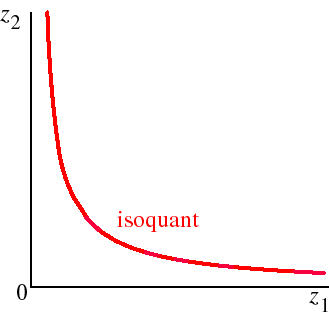
\includegraphics[width=.3\textwidth]{./Curves/CD.png}\hfill
    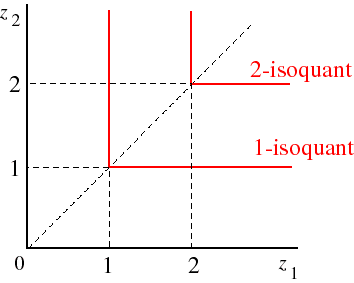
\includegraphics[width=.3\textwidth]{./Curves/C.png}\hfill
    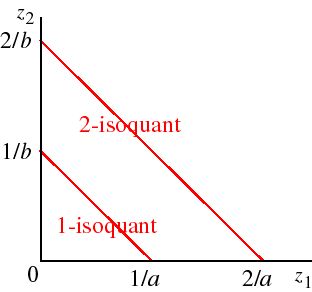
\includegraphics[width=.3\textwidth]{./Curves/S.png}  
    \caption{Utility Curves}
    \label{fig:Utility Curves} 
    \end{figure}  

\subsection{Quasilinear Utility Functions}
Utility function that is independent of the income effect. 
\begin{equation}
    u(x,y) = v(x) + y
    \notag
\end{equation}
where $v$ is an arbitrary function that is strictly increasing if good $x$ is desired. \\
Indifference curve for $\alpha$ utility level:
\begin{equation}
\begin{split}    
    &v(x) + y = \alpha  \\
    &y = \alpha - v(x)
    \notag 
    \end{split}   
\end{equation} 

Marginal rate of substitution is computed by 
\begin{equation}
    \begin{split}       
    &MRS =\frac{\partial u}{\partial x} / \frac{\partial u}{ \partial y } \\
    &\mbox{where } \frac{\partial u}{\partial x}=v'(x) \mbox{ and } \frac{\partial u}{\partial y} = 1 \\
    &\mbox{Therefore } MRS = v'(x)
    \notag
    \end{split}    
\end{equation}

\section{Slutsky decomposition: Income and substitution effects}
Slutsky decomposition is the total effect of substitution and income. 

\subsection{Normal Goods}
Normal goods are goods for which demand increases when income increases. 
In the slutsky decomposition, the income and substitution effect reinforce each other when the the good's price change. \\
Income and substitution effects cause an increase in demand when prices decrease. 

\subsection{Income Inferior Goods}
Demand reduced with higher income. \\
Substitution and Income effects oppose each other. When income increases, demand decreases, the substitution effect is the same as normal goods. 

\subsection{Griffon Goods}
Extreme income-inferiority, the income effect may be larger in size than the substitution effect, causing quantity demanded  
demanded to fall as own-prices rises. \\
Slutsky's decomposition of the effect of a price change into a pure substitution effect and an income effect thus explains why the law of downwards-slopping
demand is violated for extremely income-inferior goods.  

\section{Microeconomy}
\subsection{The intertemporal utility function}
A plan for consumption in the periods $0, 1, ... , T-1$ is denoted ${c_t}^{T-1}_{t=0}$, where $c_t$ is the consumption in period $t$. We say the plan has \underline{time horizon T}. 
Period 0 (‘the initial period’) need not refer to the ‘birth’ of the household but is just an arbitrary period within the lifetime of the household . \\

We assume that preferences of a household/consumer can be represented by a time-separable intertemporal utility function with a constant utility discount rate and no utility from 
leisure (the latter assumption implies that the labour supply curve of the household in each period is inelastic, ie whatever the changes of prices of labour and leisure the supply of labour stays the same). 
The time-separability itself just means that the intertemporal utility funciton is additive.  \\ 
In addition, we assume geometric utility discounting, meaning that utility obtained $t$ periods ahead is converted into a present equivalent by multiplying by the discount factor $(1 + q)^{-t}$, where $q$ 
is a constant utility discount rate. Hence, $u_t(c_t) = u(c_t)(1 + q)^{-t} $, where $u(c)$ is a time-independent period utility function. Together, these two assumptions amount to
$$ U(c_0, c_1, ..., c_{T-1}) = u(c_0) + \frac{u(c_1)}{(1+q)} + ... +  \frac{u(c_{T -1})}{(1+q)^{T-1}} = \sum_{t = 0}^{T - 1} \frac{u(c_{t})}{(1+q)^{t}} $$

The period utility function is assumed to satisfy $u'(c) > 0 $ and $u''(c) < 0 $.  \\ 
The number $ 1 + q$ tells how many units of utility in the next period the household insists on "in return" for a decrease of one unit of utility in the current period. 
So, a $q > 0$ will reflect that if the chosen level of consumption is the same in two periods, then the individual always appreciates a marginal unit of consumption higher the earlier it arrives. 
This explains why $q$ is named the \underline{rate of time preference} or \underline{rate of impatience}. \\ The utility discount factor, $\frac{1}{1+q}^t$, indicates how many units of utility the household is at most willing to give up 
in period 0 to get one additional unit of utility in period $t$.

Now we assume that the consumer has a utility function over consumption today (time period 0, $t = 0$) and the future (time period 1, $t = 1$). Say, 
$$ u(c_{t = 0},c_{t = 1}) = c_{t = 0}^{\alpha} + \frac{1}{1+q} * c_{t = 1}^{\alpha} $$ 
where $\alpha$ is a parameter between 0 and 1, say 0.5, and $q$ is a given number for instance 0.04. 
The consumer has some income/endowment ($e$ or $I$)in both periods but can also save or borrow money. Savings $s$ is given by 
$$ s = e_0 - c_{t = 0} $$ 
and consumption in period 2 is given by 
$$ c_{t = 1} = e_1 + s \times (1+r)$$ 
where $r$ is the interest rate ($s$ will be negative if the consumer borrows money.) Since $e_1$ is in tomorrow's money, we have to multiply the savings we bring forward by $(1 + r)$ to We can put this into our 
numerical framework by substituting for $s$, giving a budget constraint 
$$ c_{t = 1} = e_1+ (e_0- c_{t = 0}) \times (1+r)$$
\hfill
Code: Visualise the changes in consumption combination (indifference curve) when the interest rate varies. 
\begin{lstlisting}[frame=single]
def f(rs,arglist):
    e = arglist[0] ; q = arglist[1]
    for element in range(len(rs)):
    r = rs[element]

    def utility(c1, c2):
        #e = 0.5 ; q = 0.04
        return np.power(c1,e)+(1/(1+q))*np.power(c2,e)

    def utility_budget(c1, ip_list):
        I1 = ip_list[0] ; I2 = ip_list[1] ; r = ip_list[2]
        c2 = I2 + (I1 - c1)*(1+r)
        return utility(c1, c2)
        
    def demand(I1, I2, r):
        c1 = newton_max(utility_budget, 0.1, [I1, I2, r])
        c2 = I2 + (I1 - c1)*(1+r)
        return c1, c2

    def indiff_dist(c2, mylist): 
        c1 = mylist[0] ; utility_level = mylist[1]
        utitility_achieved = utility(c1,c2)
        return utitility_achieved - utility_level

    def indifference(c1, util):
        return newton_add(indiff_dist, 1, [c1,util])

    def indirect_utility(I1, I2, r):
        c11, c22 = demand(I1, I2, r)
        return utility(c11, c22)

    # initialise quantiites of good 1 (x), income (I), and prices of the two goods
    c1 = np.linspace(1,30,100) ; I1 = 10 ; I2 = 12

    # get indirect utility curve here
    utility_level = indirect_utility(I1, I2, r)
    c2 = np.zeros(len(c1))

    for idx in range(len(c1)):
        c2[idx] = indifference(c1[idx], utility_level)


    #Compute the optimal demand for each r
    dem = []
    dem= demand(I1,I2,r)    

    # plot and make nice
    plt.figure(figsize = (6,4)) ; plt.plot(c1, c2, label = f'Indifference curve with r = {np.round(r,2)}')
    plt.plot(c1, I2 + (I1 - c1)*(1+r), color = 'red', label = 'budget line')
    plt.scatter(dem[0],dem[1], label = "Optimum demand", color ='black')
    plt.text(dem[0], dem[1], '({}, {})'.format(np.round(dem[0],2), np.round(dem[1],2)))
    plt.xlabel('quantity of goods consumed today') ; plt.ylabel('quantity of good s consumed tomorow')
    plt.legend(loc = 'upper right')
    plt.title('Evolution of indifference curves when interest rates varie')
    plt.xlim(0,30) ; plt.ylim(0,30)
    plt.show()

\end{lstlisting} 
\hfill
Code: Visualise Slutsky decomposition to determine consumer's behaviour. 
\begin{lstlisting}[frame=single]
    def utility(c1, c2):
    e = 0.5 ; q = 0.04
    return np.power(c1,e)+(1/(1+q))*np.power(c2,e)

def utility_budget(c1, ip_list):
    I1 = ip_list[0] ; I2 = ip_list[1] ; r = ip_list[2]
    c2 = I2 + (I1 - c1)*(1+r)
    return utility(c1, c2)
    
def demand(I1, I2, r):
    c1 = newton_max(utility_budget, 0.1, [I1, I2, r])
    c2 = I2 + (I1 - c1)*(1+r)
    return c1, c2

def indiff_dist(c2, mylist): 
    c1 = mylist[0] ; utility_level = mylist[1]
    utitility_achieved = utility(c1,c2)
    return utitility_achieved - utility_level

def indifference(c1, util):
    return newton_add(indiff_dist, 1, [c1,util])

def indirect_utility(I1, I2, r):
    c11, c22 = demand(I1, I2, r)
    return utility(c11, c22)

def diff_indirect_utilities(income_to_be_found,longlist):
    I1 = longlist[0] ; I2 = longlist[1] ; r1 = longlist[2] ; r2 = longlist[3]
    return indirect_utility(I1, I2, r1) - indirect_utility(I1,income_to_be_found,r2)

# define the parameters
I1 = 12 ; I2 = 8 ; r1 = 0.1 ; r2 = 0.85


# Give optimal income level for period 2 when prices change
a = newton_add(diff_indirect_utilities, 1, [I1, I2, r1, r2])
# print(a)

c1 = np.linspace(0.1, 10, 100) # quantity of good today

# plot with the new budget line as well
plt.figure(figsize = (12, 8))

# budget curve 1 : Before changes
plt.plot(c1, I2 + (I1 - c1)*(1+r1), color = 'pink', label = 'budget curve 1')

# budget curve2 : After changes
plt.plot(c1, a + (I1 - c1)*(1+r2), color = 'red', label = 'budget curve with a')

# get the utility levels
u_bar = indirect_utility(I1, I2, r1) 
u_bar2 = indirect_utility(I1, I2, r2)

#print(u_bar, u_bar2)

# express utility max as a function of quantity of good tomorrow
c21 = np.zeros((100,1)) ; c22 = np.zeros((100,1))

for idx in range(len(c1)):
    c21[idx] = indifference(c1[idx], u_bar)
    c22[idx] = indifference(c1[idx], u_bar2)

plt.plot(c1, c21, label = 'indifference curve 1', color = 'green') 
plt.plot(c1, c22, label = 'indifference curve 2', color = 'blue')

# find utility-maximising consumption bundle
dems1 = demand(I1, I2, r1) ; plt.scatter(dems1[0], dems1[1],s=50,alpha=0.5,color='black')
dems2 = demand(I1, I2, r2) ; plt.scatter(dems2[0], dems2[1],s=50,alpha=0.5,color='black')

# make nice
# plt.vlines(dems1[0], 8, 10.5, linestyles = 'dotted', color = 'k')
# plt.vlines(dems2[0], 8, 10.5, linestyles = 'dotted', color = 'k')
plt.annotate('A', xy = (dems1[0], dems1[1]), xycoords='data',rotation = 30, size=15)
plt.annotate('B', xy = (dems2[0], dems2[1]), xycoords='data',rotation = 30, size=15)

plt.vlines(dems1[0],0,dems1[1],linestyles='dotted')
plt.vlines(dems2[0],0,dems2[1],linestyles='dotted')
plt.hlines(dems1[1],0,dems1[0], linestyles='dotted')
plt.hlines(dems2[1],0,dems2[0], linestyles='dotted')
plt.ylim(0,40) ; plt.xlim(0,10)
plt.title('Income and Substitution effect: Consequences on consumption in time')
plt.xlabel('consumption today, c1') ; plt.ylabel('consumption tomorrow, c2')
plt.legend(loc = 'upper right') 

\end{lstlisting}
Then to determine the consumer's behaviour you compute the savings for the first period (today). 
\begin{lstlisting}[frame=single]
s = I1 - dems1[0]
# where dems1[0] is the consumer of today's goods
\end{lstlisting}  
If the savings are negative then the consumer is a borrower, if savings are positive then the consumer is a saver. 
To visualise both cases you can play with the values of Incomes (I1 and I2) and the rates (r1 and r2).  
\end{document}

